\documentclass{article}
\usepackage{graphicx}
\usepackage{amsmath}
\usepackage{enumitem}
\usepackage{hyperref}
\usepackage{xcolor}
\usepackage{caption}
\graphicspath{ {./} }

\newcommand{\mysubsection}[1]{
    \subsubsection*{#1}
    \addcontentsline{toc}{subsection}{#1}
    \vspace{-1em}
    \rule{\linewidth}{.1mm}
    \par
}

\captionsetup{font=small,labelfont=bf,justification=centering,skip=5pt}

\begin{document}

    \pagenumbering{roman}
    \tableofcontents
    \pagebreak


    \pagenumbering{arabic}
    \begin{center}
        \subsection*{Basics}
        \addcontentsline{toc}{section}{Basics}
    \end{center}

    \medskip
    \subsubsection*{Charge, Current, Voltage, Power, and Energy}
    \addcontentsline{toc}{subsection}{Charge, Current, Voltage, Power, and Energy}
    \vspace{-1em}
    \rule{\linewidth}{0.1mm}

    \vspace{0.2em}\noindent
    Current is rate of the flow of charge through an element in a circuit.
    \[
        i = \frac{dq}{dt} \qquad Q = \int_{t_0}^t i\,dt
    \]

    \vspace{.2em}\noindent
    Voltage, or electric potential difference, is analogous to pressure.
    The difference in electric potential between two points is what causes current.
    \[
        v = \frac{dw}{dq}
    \]

    \vspace{.2em}\noindent
    Power is the rate of change of work with respect to time, measured in watts (W). Power expended or absorbed between time $t_0$ and $t$ is work.
    \[
        p = \frac{dw}{dt} = \frac{dw}{dq} \cdot \frac{dq}{dt} = vi
        \quad \Longleftrightarrow \quad
        w=\int_{t_0}^t p\,dt = \int_{t_0}^t vi \,dt
    \]

    \vspace{.2em}\noindent
    Passive sign convention dictates that when current flows into the positive terminal of an element $p = +vi$ and when current flows into the negative terminal of an element $p = -vi$.
    An element with positive power is absorbing power from the circuit; an element with negative power is supplying power to the circuit.

    \vspace{4em}
    \smallskip
    \subsubsection*{Problem-Solving}
    \addcontentsline{toc}{subsection}{Problem-Solving}
    \vspace{-1em}
    \rule{\linewidth}{0.1mm}

    \vspace{.2em}\noindent

    \begin{enumerate}[label=\arabic*.]
        \item Understand the fundamentals of the problem.
        \item Detail all relevant information.
        \item Create alternative paths forward, and assess each for their viability.
        \item Attempt a solution, then review and check for accuracy.
    \end{enumerate}


    \pagebreak
    \begin{center}
        \subsection*{Fundamental Laws}
        \addcontentsline{toc}{section}{Fundamental Laws}
    \end{center}

    \medskip
    \subsubsection*{Ohm's Law}
    \addcontentsline{toc}{subsection}{Ohm's Law}
    \vspace{-1em}
    \rule{\linewidth}{0.1mm}

    \vspace{.2em}\noindent
    Ohm's law states that the current flowing through a conductor is directly proportional to the voltage across it.
    Resistance is that constant of proportionality.
    Resistance is a material's opposition to electric current.
    \[
        v=iR
    \]

    \vspace{.2em}\noindent
    The conductance $G$ of an element is the reciprocal of its resistance:
    \[
        G = \frac{1}{R}
    \]

    \vspace{.2em}\noindent
    Using Ohm's law, we now have additional ways to express power.
    The power dissipated by a resistor can be expressed as
    \[
        p=vi=i^2 R=\frac{v^2}{R}=v^2 G=\frac{i^2}{G}
    \]

    \smallskip
    \subsubsection*{Fundamental Theorem of Network Topology}
    \addcontentsline{toc}{subsection}{Fundamental Theorem of Network Topology}
    \vspace{-1em}
    \rule{\linewidth}{0.1mm}

    \vspace{.2em}\noindent
    A \emph{branch} is a single element in an electric circuit.
    A \emph{node} is the point of connection between two or more branches.
    A \emph{loop} is a closed path in a circuit.
    The number of $b$ branches, $n$ nodes, and $l$ independent loops are related by the fundamental theorem of network topology.
    \[
        b = l+n-1
    \]

    \smallskip
    \subsubsection*{Kirchhoff's Laws}
    \addcontentsline{toc}{subsection}{Kirchhoff's Laws}
    \vspace{-1em}
    \rule{\linewidth}{0.1mm}

    \vspace{0.2em}\noindent
    Kirchhoff's current law (KCL) states that the currents at any node algebraically sums to zero; the sum of currents entering a node equals the sum of currents leaving the node.
    Kirchhoff's voltage law (KVL) states that the algebraic sum of all voltages around a closed loop is zero; the sum of voltage drops equals the sum of voltage rises.
    KCL and KVL can be expressed as
    \[
        \sum_{n=1}^N i_n =0 \qquad \sum_{m=1}^M v_m=0
    \]

    \smallskip
    \subsubsection*{Series Resistors - Voltage Division}
    \addcontentsline{toc}{subsection}{Series Resistors - Voltage Division}
    \vspace{-1em}
    \rule{\linewidth}{0.1mm}

    \vspace{.2em}\noindent
    The equivalent resistance of any number of resistors connected in series is the sum of the individual resistances.
    For $N$ resistors in series
    \[
        R_{eq} = R_1 + R_2 + \cdots + R_N = \sum_{n=1}^N R_n
    \]

    \vspace{.2em}\noindent
    Given a voltage divider with $N$ resistors in series with a voltage source $v$, the $n$th resistor $(R_n)$ will have a voltage
    \[
        v_n=\frac{R_n}{R_1+R_2+\cdots+R_N}\,v
    \]

    \smallskip
    \subsubsection*{Parallel Resistors - Current Division}
    \addcontentsline{toc}{subsection}{Parallel Resistors - Current Division}
    \vspace{-1em}
    \rule{\linewidth}{0.1mm}

    \vspace{.2em}\noindent
    The equivalent conductance of resistors connected in parallel is the sum of their individual conductances.
    \[
        G_{eq} = G_1+G_1+ \cdots + G_N \implies
        R_{eq} = ( G_1+ G_2+ \cdots+G_N )^{-1}
    \]

    \vspace{.2em}\noindent
    Given a current divider with $N$ conductors in parallel with a current source $i$, the $n$th conductor $(G_n)$ will have a current
    \[
        i_n=\frac{G_n}{G_1+G_2+\,\dots\,G_N}\,i
    \]

    \smallskip
    \subsubsection*{Wye-Delta Transformations}
    \addcontentsline{toc}{subsection}{Wye-Delta Transformations}
    \vspace{-1em}
    \rule{\linewidth}{0.1mm}

    \noindent
    Each resistor in the Y network is the product of the two adjacent $\Delta$ resistors, divided by the sum of the $\Delta$ resistors.
    Each resistor in the $\Delta$ network is the sum of the products of the Y resistors, taken two at a time, over the opposite Y resistor.

    \vspace{-.5em}
    \[
        \hspace{-2.7em} R_a=\frac{R_1 R_2+R_2 R_3+R_3 R_1}{R_1} \qquad R_1=\frac{R_b R_c}{R_a+R_b+R_c}
    \]
    \vspace{-1em}
    \begin{figure}[htbp]
        \centering
        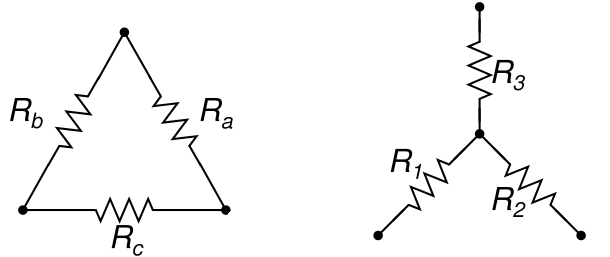
\includegraphics[width=0.5\textwidth]{wyeDelta}
        \vspace{1em}
        \caption{Wye-Delta Transformation.
        Source:
        \href{https://commons.wikimedia.org/wiki/File:Wye-delta.svg}{\color{blue}\underline{Wikipedia}}
        (\href{https://creativecommons.org/licenses/by-sa/3.0/deed.en}{\color{blue} \underline{CC BY-SA 3.0}}).}

        \label{fig:wye-delta}
    \end{figure}



    \pagebreak
    \begin{center}
        \subsection*{Nodal and Mesh Analysis}
        \addcontentsline{toc}{section}{Nodal and Mesh Analysis}
    \end{center}

    \medskip
    \subsubsection*{Nodal Analysis}
    \addcontentsline{toc}{subsection}{Nodal Analysis}
    \vspace{-1em}
    \rule{\linewidth}{0.1mm}

    \vspace{.2em}\noindent
    Steps to determine node voltages:

    \begin{enumerate}[label=\arabic*.]
        \item Select a reference node and assign voltage variables to the remaining nodes.
        \item If there is a voltage source between the reference node and another node, the non-reference node's voltage is equal to that of the voltage source.
        \item If there is a voltage source between two non-reference nodes, those two nodes form a supernode, so we and apply both KCL and KVL\@.
        \item Apply KCL to each node with an unknown voltage.
        \item Use Ohm's law to express the branch currents in terms of voltage.
        In a resistor, current flows from a higher potential to a lower potential.
        \[
            i = \frac{v_{\text{ higher}} - v_{\text{ lower}}}{R}
        \]
        \item Solve the resulting system of equations.
    \end{enumerate}

    \smallskip
    \subsubsection*{Mesh Analysis}
    \addcontentsline{toc}{subsection}{Mesh Analysis}
    \vspace{-1em}
    \rule{\linewidth}{0.1mm}

    \smallskip\noindent
    A loop is a path in which no node is passed more than once.
    A mesh is a loop that does not contain any other loops within it.
    Mesh analysis only works for circuits that are planer, i.e., they can be drawn on a plane without crossing branches.

    \begin{enumerate}
        \item Assign mesh currents to each mesh.
        \item When a current source is only in one mesh it defines the mesh current.
        \item When a current source is between two meshes, create a supermesh by excluding the current source and any elements connected in series with it.
        We apply both KVL and KCL to the supermesh.
        \item Apply KVL to each of the meshes, using Ohm's law to express the voltages in terms of mesh currents.
        \item Solve the resulting system of equations.
    \end{enumerate}

    \pagebreak
    \begin{center}
        \subsection*{Circuit Theorems}
        \addcontentsline{toc}{section}{Circuit Theorems}
    \end{center}

    \smallskip
    \mysubsection{Linearity and the Principle of Superposition}

    \smallskip\noindent
    The following theorems apply only to linear circuits.
    Basically, a linear circuit is a circuit whose output voltage and current are linear functions of its input voltage and current.
    More specifically, a linear circuit is one that follows the principle of superposition, i.e.\ has the characteristics of additivity and homogeneity.

    Additivity: the voltage across and current through an element is equal to the algebraic sum of each voltage and current source applied to the element individually.

    Homogeneity: scaling the input sources by a factor $k$ scales the output by a factor $k$.
    \vspace{-.5em}
    \begin{gather*}
        f(x_1+\dots+x_n) = f(x_1)+\dots+f(x_n)  \\[.3em]
        f(k\,x)=k\,f(x)
    \end{gather*}

    \smallskip\noindent
    The principal of superposition can be directly applied to find voltages or currents of a given element without solving the rest of the circuit; however, it is often times mathematically more simple to solve the whole circuit.


    \smallskip
    \subsubsection*{Source Transformation}
    \addcontentsline{toc}{subsection}{Source Transformation}
    \vspace{-1em}
    \rule{\linewidth}{0.1mm}

    \smallskip\noindent
    A voltage source in series with a resistor may be replaced by a current source in parallel with that resistor.
    A current source in parallel with a resistor may be replaced by a voltage source in series with that resistor.
    When transforming voltage to current, the current flows out of the positive terminal.
    When transforming current to voltage, the resistor is placed on the positive side of the voltage source.
    This can be applied to both independent and dependent sources.
    Figure~\ref{fig:thev-norton-transf} shows these configurations.

    Source transformation cannot be applied to a short circuit or open circuit.
    Following Ohm's law, the transformed source takes on a value as defined below.

    \[
        v_s = i_s R     \qquad   i_s = \frac{v_s}{R}
    \]

    \smallskip
    \subsubsection*{Thevenin's Theorem and Norton's Theorem}
    \addcontentsline{toc}{subsection}{Thevenin's Theorem and Norton's Theorem}
    \vspace{-1em}
    \rule{\linewidth}{0.1mm}

    \smallskip\noindent
    From the perspective of two terminals, any linear circuit behaves as though it comprises only a voltage source in series with a resistor (Thevenin equivalent circuit) or comprises only a current source in parallel with a resistor (Norton equivalent circuit).

    The Thevenin or Norton equivalent resistance ($R_\text{Th} = R_\text{N}$) are found by removing all independent voltage and current sources from a circuit, then calculating the equivalent resistance.
    If there are dependent sources, leave them in place and solve for the equivalent resistance by injecting $v_0$ = 1\,V or $i_0$ = 1\,A (for easy calculations) at the target terminals.
    Solve for the resulting current or voltage, and $R_\text{Th} = R_N = v_0/i_0$

    Thevenin equivalent voltage ($V_\text{Th}$) is found by solving for the voltage between the target terminals, i.e., the voltage at the open circuit.
    Norton equivalent current ($I_N$) is found by solving for the current between the terminals if they were to be short-circuited.

    Figure~\ref{fig:thev-norton-transf} shows the end result of simplifying a linear circuit to its Thevenin equivalent or Norton equivalent.
    It is worthwhile to note that each is a source transformation of the other.

    \begin{figure}[htbp]
        \centering
        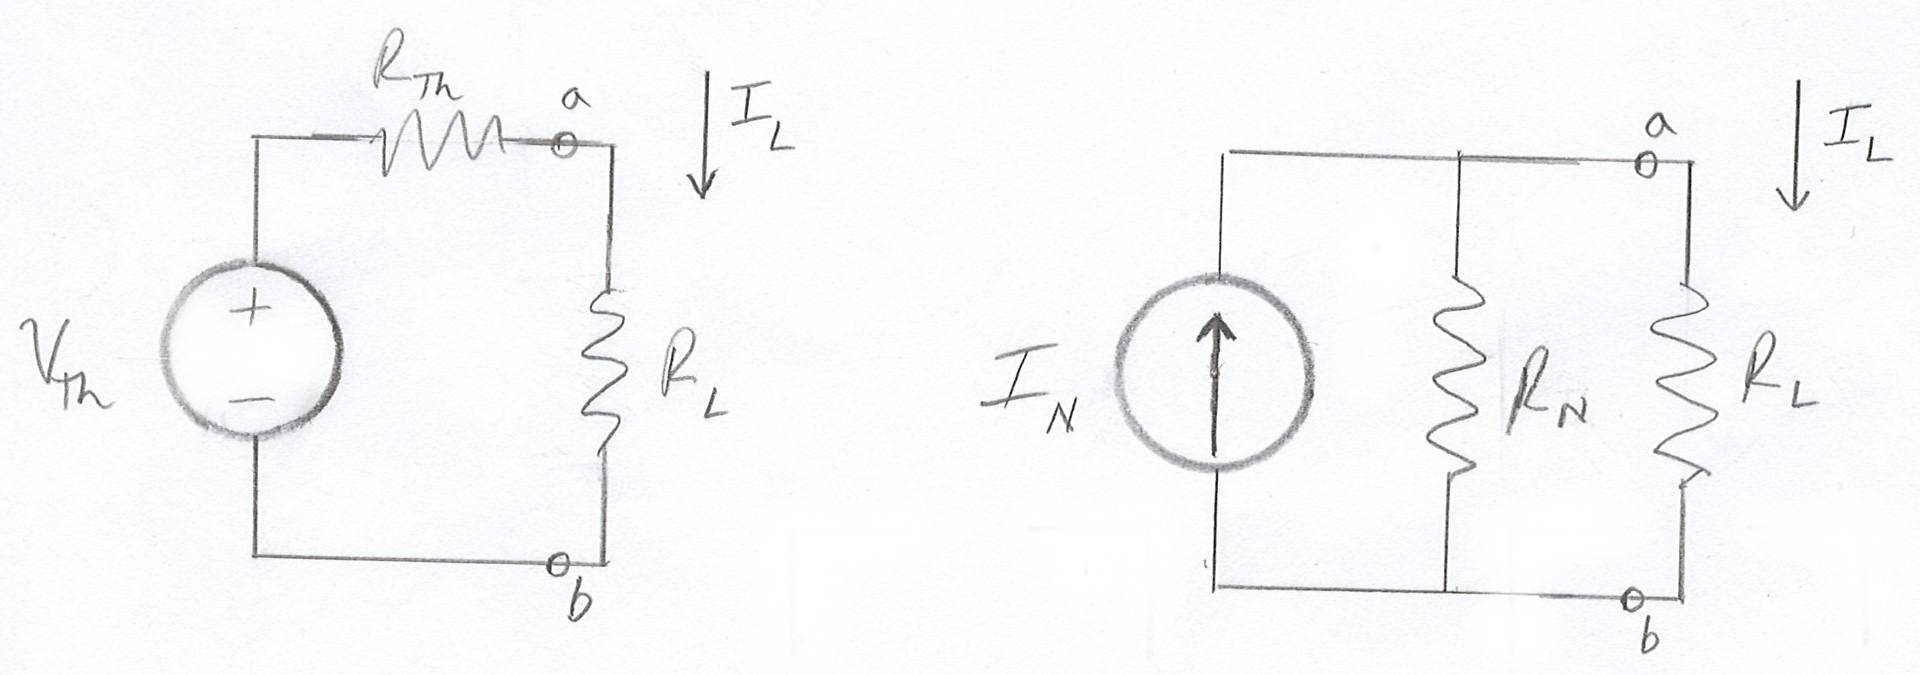
\includegraphics[width=.7\textwidth]{theveninNortonTransform}
        \caption{Thevenin and Norton Equivalent Circuits. \\
        Source:
        \href{https://github.com/de-Manzanares}
        {\color{blue}\underline{de-Manzanares}}
        (\href{https://creativecommons.org/licenses/by-nc-sa/4.0/deed.en}{\color{blue} \underline{CC BY-NC-SA 4.0}}).}

        \label{fig:thev-norton-transf}
    \end{figure}

    \smallskip\noindent
    Following Ohm's law, the principle of voltage division, and the principle of current division, the load characteristics (voltage, current, and resistance) are related to a circuit's Thevenin and Norton equivalents as follows:
    \begin{gather*}
        I_L = \frac{V_{\text{Th}}}{R_{\text{Th}}+R_L}
        \qquad
        V_L = I_L R_L = \frac{V_\text{Th}R_L}{R_{\text{Th}}+R_L}    \\[.5em]
        I_L = \frac{R_L^{-1}}{R_N^{-1}+R_L^{-1}}\,I_N
        \qquad
        V_L = I_L R_L = \frac{I_N}{R_N^{-1} + R_L^{-1}}
    \end{gather*}

    \medskip
    \noindent
    If a circuit contains dependent sources it is possible for the Thevenin equivalent resistance to be negative.
    This means that the circuit is supplying power to the terminals.

    \smallskip
    \mysubsection{Power Transfer}
    \smallskip
    \noindent
    Solving $dp/dR_L = 0$ gives $R_L=R_\text{Th}$, meaning that maximum power transfer occurs when the load resistance is equal to the Thevenin equivalent resistance.
    The following equations express power of a circuit for any $R_L$ and for the special case $R_L = R_\text{Th}$, respectively.
    \begin{gather*}
        p=\left( \frac{V_{\text{Th}}}{R_{\text{Th}}+R_L} \right) ^2 R_L \qquad
        p_\text{max} = \frac{V_\text{Th}^2}{4R_\text{Th}}
    \end{gather*}

\end{document}
